% Figure from MATH 493 notes, section 56 (the grid Z_ij = X_i cap Y_j). From WS 12 (orientation of the worksheet and the board: j increases upward).
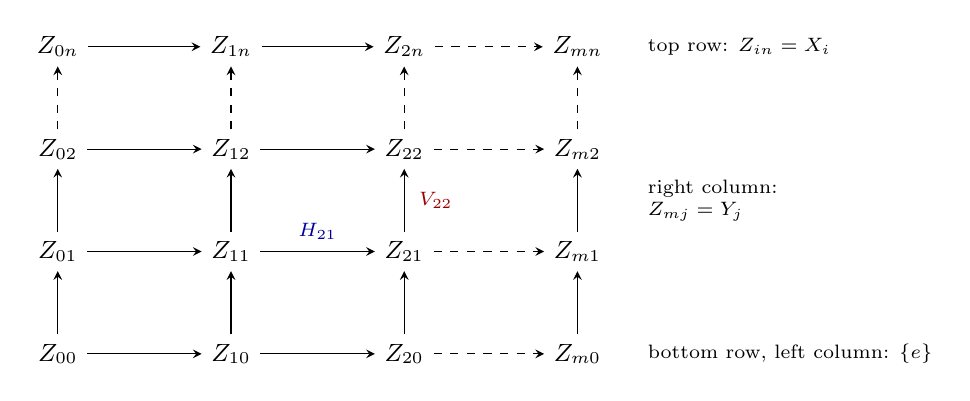
\begin{tikzpicture}[x=2.2cm, y=1.3cm, font=\small, >=stealth]
  \foreach \i/\li in {0/0, 1/1, 2/2, 3/m} {
    \foreach \j/\lj in {0/0, 1/1, 2/2, 3/n} {
      \node (z\i\j) at (\i, \j) {$Z_{\li\lj}$};
    }
  }
  \foreach \j in {0,1,2,3} { \draw[->] (z0\j) -- (z1\j); \draw[->] (z1\j) -- (z2\j); \draw[->, dashed] (z2\j) -- (z3\j); }
  \foreach \i in {0,1,2,3} { \draw[->] (z\i0) -- (z\i1); \draw[->] (z\i1) -- (z\i2); \draw[->, dashed] (z\i2) -- (z\i3); }
  \node[above, font=\scriptsize, blue!60!black] at (1.5, 1.02) {$H_{21}$};
  \node[right, font=\scriptsize, red!60!black] at (2.03, 1.5) {$V_{22}$};
  \node[font=\scriptsize, anchor=west, align=left] at (3.35, 3) {top row: $Z_{in} = X_i$};
  \node[font=\scriptsize, anchor=west, align=left] at (3.35, 1.5) {right column:\\ $Z_{mj} = Y_j$};
  \node[font=\scriptsize, anchor=west, align=left] at (3.35, 0) {bottom row, left column: $\{e\}$};
\end{tikzpicture}
